\lecture{22}{9 maggio 2024}
\paragraph{Reticolo}
Un reticolo è un dispositivo caratterizzato da un numero N di fenditure grandi. Detto \(N^{\prime} \) il numero di fenditure per unità di lunghezza, si ha \(d= \quotient{1}{N^{\prime} } \). Per il reticolo si definisce la dispersione, che è la capacità di deviare la luce al variare della lunghezza d'onda: \(\mathcal{D} = \frac{\mathrm{d}\theta }{\mathrm{d} \lambda } = \frac{m}{d \cos (\theta_{max})} \) usando la formula dei massimi. Si definisce anche il potere risolutivo \(\mathcal{R} =\frac{\lambda }{\mathrm{d}\lambda } \) come la capacità di vedere come separati massimi a lunghezze d'onda molto vicine. Quindi non conta solo la distanza fra i picchi ma anche quanto è largo un picco. Considerato \(\mathrm{d} \theta \thickapprox \Delta \theta = \frac{\lambda }{N d}\) come distanza angolare fra i picchi, otteniamo
\begin{equation}
	\mathcal{R} = \frac{\lambda }{\mathrm{d} \lambda } = \frac{Nm}{\cos (\theta_{max})} \thickapprox Nm
\end{equation}

\begin{note}
	Nelle slide ci sono esempi di applicazioni dell'interferenza con film sottili (L30).
\end{note}

\section{Diffrazione}
Il fenomeno fisico alla base del fenomeno della diffrazione è lo stesso dell'interferenza. Si parla di diffrazione quando ho un numero "infinito" di sorgenti distribuite su un'apertura. Si applica il principio di Huygens-Fresnel a un'onda monocromatica piana che incide su una fenditura di larghezza \(a\):
\begin{figure}[H]
	\centering
	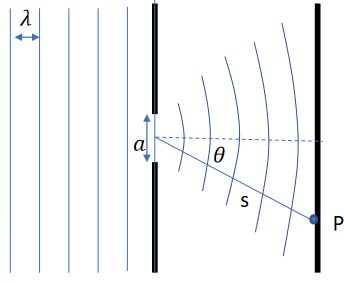
\includegraphics[width=0.35\textwidth]{screenshots/2024-05-09-10-18-53.png}
\end{figure}
Ci sono condizioni più semplici per il calcolo della figura di diffrazione e altre più complicate. Se lo schermo su cui si osserva la figura è vicino all'apertura si parla di diffrazione in regime di Fresnel, se è lontano si parla di regime di Fraunhofer e si usa l'approssimazione per angoli piccoli. Usiamo la descrizione matematica del principio di Huygens-Fresnel:
\begin{figure}[H]
	\centering
	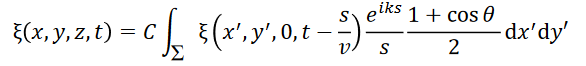
\includegraphics[width=0.4\textwidth]{screenshots/2024-05-09-10-22-24.png}
\end{figure}
Ci poniamo in questa situazione:
\begin{figure}[H]
	\centering
	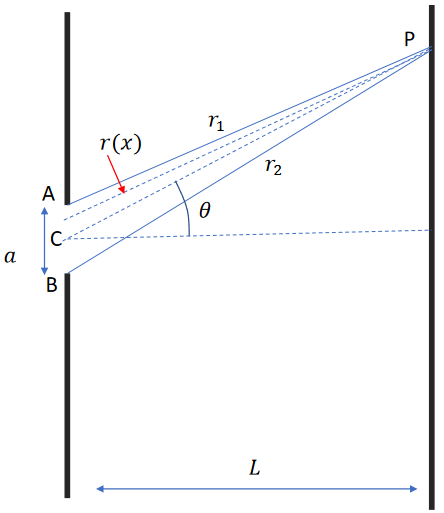
\includegraphics[width=0.3\textwidth]{screenshots/2024-05-09-10-22-53.png}
\end{figure}
In prima approssimazione considero l'onda perpendicolare alla fenditura, quindi il campo elettrico è uniforme sull'apertura: \(\vec{E}(x)= E_0 e^{-i \omega t} \vec{\hat{n}}\). In prima approssimazione il campo in P è dato dalla sovrapposizione di tutti i campi provenienti dai diversi punti dell'apertura: \(\vec{E}(P)= C \int E_0^{\prime} e^{i(kr(x)- \omega t)}\mathrm{d} x\). Per angoli piccoli posso scrivere \(r_2 - r_1 = a \sin (\theta )\), quindi la differenza di fase fra i due raggi è dovuta alla differenza di cammino ottico: \(\Delta \varphi = ka \sin (\theta )\).
\begin{figure}[H]
	\centering
	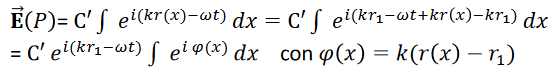
\includegraphics[width=0.4\textwidth]{screenshots/2024-05-09-10-28-32.png}
\end{figure}
Consideriamo il caso particolare in cui \(\Delta \varphi = \varphi (B) - \varphi (A) = ka \sin (\theta ) = 2\pi \). L'integrale è fatto su tutte le fasi intermedie fra \(0\) e \(2\pi \), quindi è nullo. Ne consegue che \(\vec{E}(P^{\star} )=0\). Abbiamo trovato dei minimi di intensità:
\begin{equation}
	\sin (\theta_{min} )=n \frac{\lambda }{a} \text{ con } n= \pm 1, \pm 2, \dots, \pm \infty 
\end{equation}
\begin{note}
	Si noti che nell'interferenza la stessa condizione si applica ai \textbf{massimi}.
\end{note}
Si esclude il caso \(n=0\) perché in tal caso tutte le onde arrivano in fase sullo schermo e quindi si ha interferenza costruttiva. Calcoliamo più precisamente l'intensità (applicando comunque delle approssimazioni):
\begin{equation}
	E(P,t) \thickapprox C \int_{-\frac{a}{2}}^{\frac{a}{2}} E_0 e^{-i \omega t} \frac{e^{i k s}}{s} \,\mathrm{d}x 
\end{equation}
Sia \(s_0 =r_0\) la distanza tra C e P. Sia r la distanza di un punto di ascissa x generica con il punto P. Si ha che \(s(x) = r_0 - x \sin (\theta )\). Al numeratore la variabilità di s con x è importante, mentre al denominatore è trascurabile. % TODO: ma perché?
\begin{figure}[H]
	\centering
	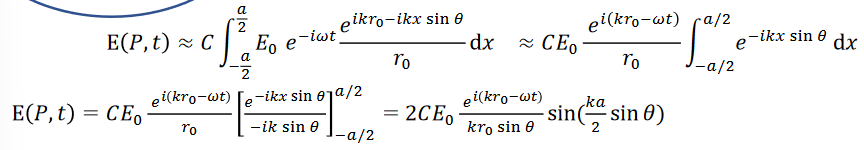
\includegraphics[width=0.4\textwidth]{screenshots/2024-05-09-10-40-03.png}
\end{figure}
Sia \(\alpha = ka \sin (\theta )\) lo sfasamento dei raggi estremi.
\begin{figure}[H]
	\centering
	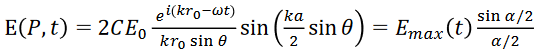
\includegraphics[width=0.4\textwidth]{screenshots/2024-05-09-10-42-12.png}
\end{figure}
Di conseguenza si ha l'espressione dell'intensità rispetto all'angolo:
\begin{equation}
	I(\theta )=
	I_0 \frac{\sin ^{2} \left( \frac{\alpha}{2} \right) }{\left( \frac{\alpha}{2} \right) ^{2} }=
	I_0 \frac{\sin ^{2} \left( \frac{ka \sin (\theta )}{2} \right) }{\left( \frac{ka \sin (\theta )}{2} \right) ^{2} }
\end{equation}
La distanza fra i due minimi vicini è \(\Delta \theta = 2 \quotient{\lambda }{a} \), quindi la larghezza del massimo centrale a circa metà altezza è \(\Delta \theta = \quotient{\lambda }{a} \).

\subsection{Diffrazione da foro circolare}
Consideriamo un foro circolare di diametro D su uno schermo e un'onda armonica piana incidente normalmente.
\begin{figure}[H]
	\centering
	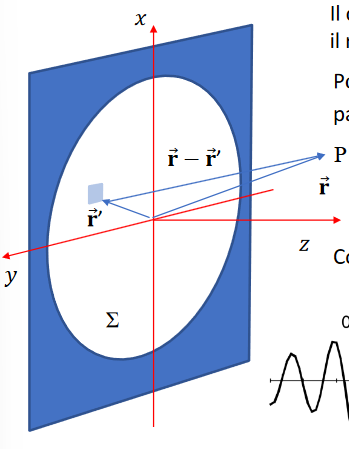
\includegraphics[width=0.3\textwidth]{screenshots/2024-05-09-10-46-54.png}
\end{figure}
In regime di Fraunhofer è risolvibile, in regime di Fresnel è necessario affidarsi a un computer. Posto \(\alpha = \frac{kD}{2}\sin (\theta )\) lo sfasamento tra un raggio che parte dal centro e uno dal bordo, si ha
\begin{figure}[H]
	\centering
	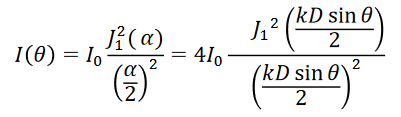
\includegraphics[width=0.3\textwidth]{screenshots/2024-05-09-10-48-05.png}
\end{figure}
dove \(J_1(\alpha )\) è una funzione di Bessel di ordine 1. Il primo minimo si ottiene a \(\sin (\theta ) = 1.22 \frac{\lambda }{D}\), quelli successivi non sono equispaziati (la funzione di Bessel non è periodica). Applichiamo quanto trovato a un occhio umano. Se guardiamo una sorgente puntiforme monocromatica attraverso un buco di uno spillo (\(D\thickapprox \SI{0.5}{mm}\)), sulla retina si forma la figura di diffrazione:
\begin{figure}[H]
	\centering
	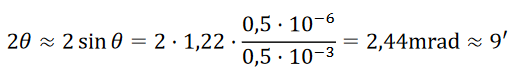
\includegraphics[width=0.35\textwidth]{screenshots/2024-05-09-10-52-56.png}
\end{figure}

\paragraph{Principio di Babinet} In regime di Fraunhofer, la figura di diffrazione prodotta da un disco opaco di diametro D è identica a quella di una apertura circolare di diametro D prodotta su uno schermo opaco.

\paragraph{Bright spot}
Poisson era un sostenitore della teoria corpuscolare e sosteneva che, se fosse stata vera la teoria ondulatoria, allora dietro ad un disco opaco si sarebbe dovuto vedere un punto illuminato al centro dell'ombra anche in regime di Fresnel. Plot twist: c'è davvero.

\paragraph{Potere separatore}
Se ho due sorgenti puntiformi incoerenti (quindi no interferenza), devo avere un potere separatore sufficiente perché il massimo di una delle due intensità sia nel punto di minimo dell'altra.
\begin{figure}[H]
	\centering
	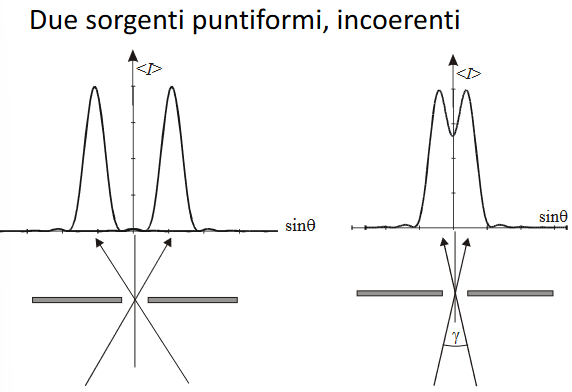
\includegraphics[width=0.4\textwidth]{screenshots/2024-05-09-10-58-57.png}
\end{figure}
Si definisce separazione \(\gamma _R = 1.22 \frac{\lambda }{D}\) e potere separatore (o risolutivo, o risoluzione): \(\frac{1}{\gamma _R} = \frac{D}{1.22 \lambda }\). Nell'occhio umano si ha
\begin{figure}[H]
	\centering
	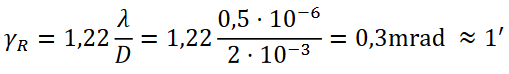
\includegraphics[width=0.4\textwidth]{screenshots/2024-05-09-11-01-31.png}
\end{figure}